\chapter{Anomaly Detection}\label{chap:AD}
\section{What is it?}\label{sec:WhatisAD}
Normally, search paradigms in Particle Physics use to investigate collisions happening at the LHC target a specific physical model. This approach has a limited field of application and so far it showed being ineffective to find New Physics (NP). There are two possible reasons behind this failure: there is no New Physics at current LHC energy or "traditional" search paradigms are not efficient with NP. At this point it is time to try something different in order to hope to understand something more about Beyond Standard Model phenomena: Anomaly Detection could be the solution.\\
When applying Anomaly Detection \cite{DLforAD}\cite{LHCOlympics}, we are looking for outliers or rare events, which typically have a small deviation from already known events. In this case data is divided into two categories: "background", containing Standard Model events or noise, and "signal", including the hypothetical New Physics. All SM phenomena are classified within background without any distinction based on the origin of data. It is now possible to understand why Anomaly Detection is defined "model agnostic": in fact it does not rely on a specific theoretical model. This feature allows to scan a bigger range of events but it is less sensitive to any specific model. \\

\begin{figure}[h!]
    \centering
    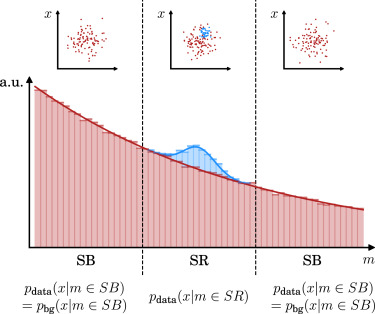
\includegraphics[width=2 in]{OLD/Images/Cap3/BumpHint.png}
    \caption{Search for anomalies in particle physics. Figure from Ref. \cite{ML4ADHEP}}
    \label{fig:bumphint}
\end{figure}

\noindent To understand Anomaly Detection, we can use an example. Assuming we need to find a church in a town we do not know, without any technology. Instead of desperately walking around, we decide to climb an hill where we can scan the whole town with not so much effort. It is possible to identify the neighbourhood of the church or the "spatial region" where it is situated. We can also get some information we would not have got in the town, such as the colour of the roof or of the facade of the building we are looking for. Then we climb down the hill and go straight to the point we observed. Thanks to the details we obtained up there, we are able to find the church quite quickly and more easily. In other words, the church represents New Physics, climbing the hill is Anomaly Detection, climbing down is using normal data analysis techniques. It is quite powerful, isn't it? To apply Anomaly Detection it is necessary to hypothesize that anomalies are rare and they represent a small portion of a whole dataset. This assumption is realistic because it is what happens everyday in airports, finance and particle physics: normal events are way more common then deviations. In addition, if anomalies in Particle Physics were more frequent, we would have already observed them through common data analysis.

%%%%%%%%%%%%%%%%%%

\section{Deep Learning and Anomaly Detection}\label{sec:DLforAD}
While working on a Particle Physics problem, it is common to deal with a huge amount of data collected during collisions at the LHC. Machine Learning (ML) algorithms, which are able to learn from past by using vast datasets, can help in this sense. Among all categories of ML, Deep Learning (DL) is the best for our task \cite{LHCOlympics}. Based on a multi-layer Neural Network, DL can build complex data representation, which is optimal when dealing with high-dimensional dataset. Furthermore due to its implementation, that will be discussed in chapter \ref{chap:Model}, it can be exploited for model agnostic applications. \cite{ML4ADHEP}\\
ML and DL methods can be classified based on how the labels of data are used to train models. Main categories are: Supervised Learning, Unsupervised Learning and Semi-Supervised Learning.\cite{DLforAD}\\
In Supervised Learning, shown in figure \ref{fig:SUPtrain}, labeled data is used to train DL models and it can be implemented only with sufficient normal and anomalous data.

\begin{figure}[h!]
    \centering
    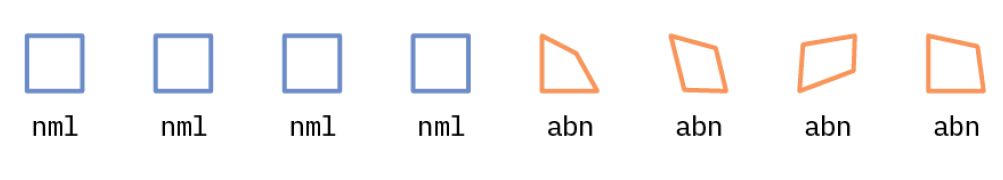
\includegraphics[width=3.5 in]{OLD/Images/Cap3/SUPtraining.png}
    \caption{Data used for Supervised Learning. Figure from Ref. \cite{DLforAD}}
    \label{fig:SUPtrain}
\end{figure}

\noindent Unsupervised Learning is based on not labeled data, as shown in figure \ref{fig:UNSUPtrain}, and models implementing it are trained to find a structure among the input features. Then model performance is tested using a mixed dataset containing both background and signal data.\\
Semi-Supervised Learning is a hybrid of previous techniques, implemented in the most varied ways.

\begin{figure}[h!]
    \centering
    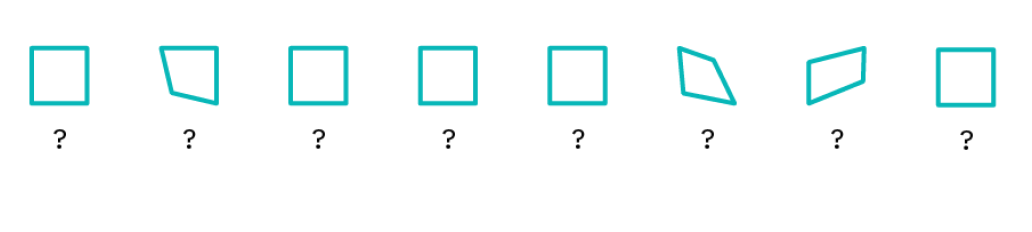
\includegraphics[width=2.7 in]{OLD/Images/Cap3/UNSUPtraining.png}
    \caption{Data used for Unsupervised Learning. Figure from Ref. \cite{DLforAD}}
    \label{fig:UNSUPtrain}
\end{figure}

\noindent In this project we implemented an Unsupervised Anomaly Detection, because labels have not been used and model was trained only over background data.

%%%%%%%%%%%%%%%%%%%%%%
\section{How is it implemented?}\label{sec:ADimplementation}
The process of training a  DL model is divided into three main phases: training, validation and test loop. They are defined "loop" because in each of them a different section of the dataset is used and the code loops over it.\\
The most important stage is the training loop: in our case the chosen DL model is trained to reconstruct arrays containing information about particle jets, using only data with normal behaviour (background events) \cite{DLforAD}. In this phase, parameters of the model are adjusted in order to best fit to data. By doing so, DL model is able to recognise very well normal data and their structure. Our hope is that, once it faces an anomaly (signal event), it is able to identify it due to its difference from what it knows. The second step is the validation loop, where a valuation of the performance of the model is elaborated using the validation set. The valuation and the search for the best weights of the model are executed computing distance between output and input over training and validation set. When this distance is minimum within the validation loop, we save the model's weights.\\
The trained and tuned model is then tested, using a dataset containing unseen data, the test set, where there are both background and signal events. The purpose of this phase is to validate results previously obtained and get a preview of what will happen once the model will be running with completely new data. The task is completed computing the Anomaly Score (AS). In this thesis, we implement it as a distance between input and output, with different dimension: instead of calculating it over a batch of data, we do so for each event. In this way we are able to plot a reconstruction probability graph: we expect that the distributions of AS from background and signal events are different, because signal data contains anomalies which our model does not know. By means of these distributions we can identify a threshold of separation between them. For any event we pass to our trained model, we compute AS: if it higher (lower) than the chosen threshold, we are looking at a background (signal) event. Since AD is distinguishing signal events from background, we are basically executing a classification task with two classes. Implementation of Anomaly Detection is discussed more in depth in chapters \ref{chap:Model} and \ref{chap:Results}.

\begin{figure}[h!]
    \centering
    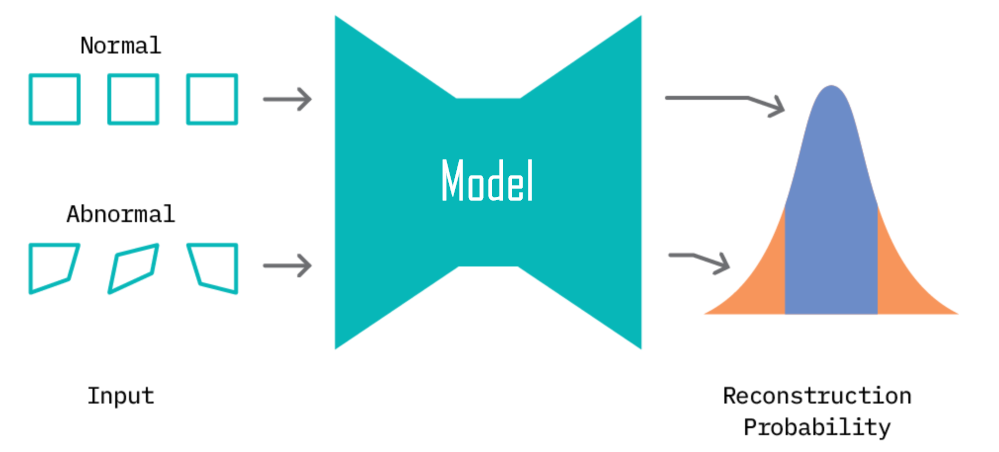
\includegraphics[width=3 in]{OLD/Images/Cap3/ADtestloop.png}
    \caption{Test loop of Anomaly Detection. Figure from Ref. \cite{DLforAD}}
    \label{fig:RECOprob}
\end{figure}


